\chapter{Implementación del sistema operativo}

Una vez que sabemos las decisiones tomadas y las tecnologías utilizadas, pasemos a estudiar cada una de las soluciones implementadas en confrontación con los requisitos estudiados.\\

Empezaremos por la puesta a punto del sistema de compilación y continuaremos con la configuración necesaria para el funcionamiento esperado del sistema operativo embebido. Dado el volumen del proyecto Yocto, describiremos solo parcialmente sus factores de configuración y el proceso de trabajo con él.

\section{Introducción y puesta a punto}

Como venimos mencionando a lo largo de la memoria, el proyecto Yocto se basa en la herramienta \textit{Open Embedded} y en el lenguaje de configuración \textit{Bitbake}, que permite ajustar desde parámetros del kernel hasta elegir paquetes que no se quiere sean instalados. Además, cabe destacar que se pueden compilar imágenes con Yocto de diversas formas, ya sea utilizando contenedores aislados (a modo de máquinas virtuales) o nuestro propio sistema Linux \textit{anfitrión}, como vemos en la documentación de inicio \cite{yocto-project-quick-start-build-system}. Por mi parte, siempre he preferido hacerlo en el propio sistema, dado que así se destinan a la compilación el 100\% de los recursos asignados disponibles y el tiempo de espera es menor.\\

Para el caso que nos ocupa, la versión utilizada del proyecto Yocto ha sido la \textbf{2.4} (de nombre \textit{Rocko}), dado que se trataba de la versión estable más avanzada en el momento del desarrollo.\\

La guía relativa a la puesta a punto la encontramos en el manual \textit{Quick Start} de la web \cite{yocto-project-quick-start} ya mencionado, y consiste principalmente en instalar las dependencias necesarias para nuestra distribución y clonar mediante \texttt{git} el núcleo del proyecto, llamado \textit{Poky}, con el comando siguiente (la opción \texttt{-b} elige la rama deseada):

\begin{center}
\texttt{git clone git://git.yoctoproject.org/poky -b rocko}
\end{center}

\subsection{Manipulación y compilación de prueba}

Una vez tenemos el núcleo, lo siguiente es empezar a configurar el resultado que queremos obtener. Si ejecutamos el comando \texttt{source oe-init-build-env}, se nos generará un directorio destino \textit{build} con una configuración de ejemplo para una máquina \textit{Qemu} de 32 bits.\\ 

La premisa de este tipo de sistemas de desarrollo es incluir lo mínimo para funcionar, y que sea el desarrollador quien elija las dependencias a incluir. Por tanto, aunque dicho archivo de configuración es grande, se trata de mucho código de ejemplo y comentarios de ayuda al recién llegado.\\

Aquí podemos elegir entre cambiar el dispositivo de destino y los paquetes a instalar, o seguir adelante con una imagen mínima de prueba de la siguiente forma:

\begin{center}
\texttt{bitbake core-image-minimal}
\end{center}

El nombre \texttt{core-image-minimal} hace referencia a la imagen de menor tamaño por defecto, por lo que para hacer pruebas es suficiente. \\

\subsection{Variables de configuración del sistema}

La sintaxis de configuración es sencilla, y sigue la forma: 

\begin{center}
	\texttt{PARÁMETRO\_CONFIGURACIÓN = "valor deseado"}
\end{center}

En el directorio \textit{build} antes creado, podremos ir incorporando configuración al archivo \textit{conf/local.conf} con dicha sintaxis de la herramienta \textit{Bitbake} para instalar/borrar paquetes del dispositivo.\\

La sintaxis de código para añadir dependencias sería la siguiente (hemos de añadir esta línea al archivo \textit{conf/local.conf} mencionado):

\begin{center}
\texttt{IMAGE\_INSTALL\_append = `` <paquete1> <paquete2> ...''}
\end{center}

Si quisiéramos eliminar alguno de los paquetes incluidos por alguna librería necesaria, es tan fácil como sustituir \texttt{append} por \texttt{remove}.\\

Por otro lado, si profundizamos en los archivos de configuración descargados de cualquiera de los layers, encontramos en alguna ocasión configuración de la forma:

\begin{center}
\texttt{VARIABLE ?= "valor"}
\end{center}

Cuando un símbolo de interrogación acompaña a esta variable, significa que es un \textbf{valor por defecto}, fácilmente anulable por una asignación sin dicho símbolo en cualquier parte.\\

Por ejemplo, en la configuración por defecto, el dispositivo por destino se muestra tal que así:

\begin{center}
\texttt{MACHINE ?= "qemux86"}
\end{center}

En nuestro caso, borraremos la interrogación y escribiremos ``raspberrypi3'' entre comillas, dado que es nuestro dispositivo elegido (podemos consultar el listado completo en \href{http://layers.openembedded.org/layerindex/branch/master/machines/?q=&browse=1}{OpenEmbedded Layer Index}, junto con los layers necesarios para cada máquina).\\

\subsection{Layers y librerías}

Por otro lado, la forma de reutilizar librerías y capas ya existentes es sencilla. Podemos encontrar la lista completa de capas y paquetes pertenecientes a éstas en la referencia \cite{yocto-layers-list}. Para empezar basta con descargarlas (también mediante \texttt{git}) en el directorio raíz del sistema de compilación. Acto seguido, añadimos una línea en el fichero \texttt{./build/conf/bblayers.conf} con la ruta a la librería descargada. [\textit{bblayers} toma su nombre por \textit{Bitbake Layers}.] Hecho esto, el comando \texttt{bitbake} detectará todos los paquetes y dependencias que tenemos importados en el sistema, viéndose esto reflejado en cada compilación.\\

En la web antes mencionada, \url{https://layers.openembedded.org}, dentro de la sección \textbf{\textit{Recipes}} podemos buscar paquetes que nos interesen, dando con la(s) capa(s) que los incluyen. Por ejemplo, si quisiéramos utilizar \textit{PSplash}, una herramienta para imprimir imágenes de carga embebidas, obtendríamos lo siguiente:

\begin{figure}[H]
	\centering
	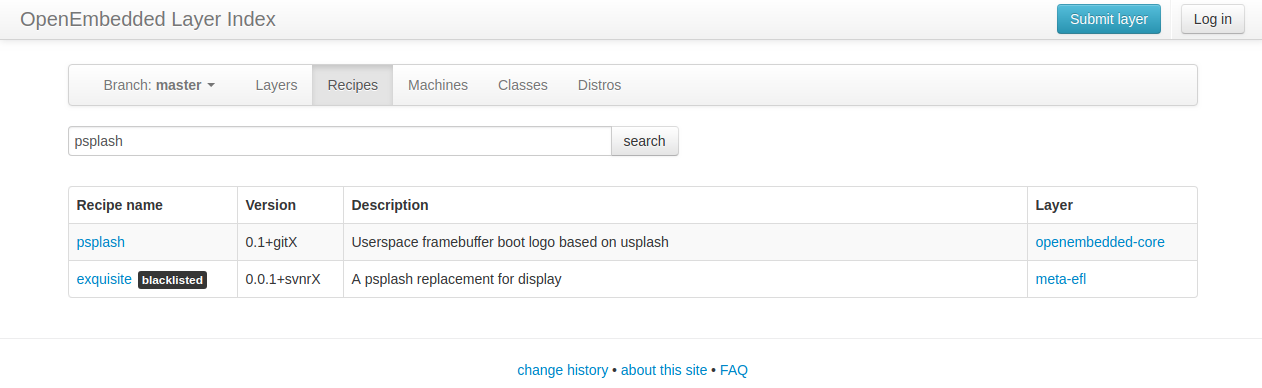
\includegraphics[width=\linewidth]{imagenes/yocto-recipe-search-example.png}
	\caption{Ejemplo de búsqueda en las recetas de OpenEmbedded [13/06/2018]}
	\label{yocto-recipe-search-example}
\end{figure}

Como vemos, los resultados vienen compuestos del nombre de los paquetes, las versiones (para filtrar cuando existen varias del mismo), una descripción inteligible y el layer donde encontrarlo. Si hacemos click en el nombre del layer, veremos una descripción de dicha capa y la dirección del repositorio donde se aloja (y que habremos de clonar).\\

\subsubsection{Layer propio}

Como aconsejan en la propia documentación de Yocto, una vez que queremos pasar de hacer pruebas a confeccionar nuestro producto, lo idóneo es \textbf{crear un \textit{layer} propio} en el que alojar la configuración de forma aislada. Por ejemplo, en nuestro caso la capa usada recibe el nombre de \texttt{meta-dynasystem} y da nombre a este proyecto.\\

Los pasos para crear un layer, descritos en la propia \textit{Wiki} de Yocto \cite{wiki-yocto-own-layer}, son sencillos. El proceso consiste básicamente en generar un par de carpetas y un archivo de configuración común al layer, describiendo las rutas internas a la capa y la prioridad de sus paquetes con respecto a los de otras.\\

\subsection{Paquetes, configuración y parches}

Para terminar con la introducción a Yocto, cabe destacar la importancia de \textbf{los parches} (o \textit{patches} en inglés). Estos permitirán de una forma escalable y, sobre todo automatizada, modificar el comportamiento de las aplicaciones y programas libres ya presentes en los repositorios.\\

Para entender el funcionamiento de los parches, veamos los estados por los que pasa un paquete por compilar:

\begin{enumerate}
	\item Se descarga el código fuente de la aplicación. El repositorio desde el que se descarga vendrá especificado por el fichero \textbf{\textit{``receta.bb''}} propio del paquete. Por ejemplo, \href{http://cgit.openembedded.org/openembedded-core/tree/meta/recipes-core/psplash/psplash_git.bb?h=master}{\texttt{la receta del paquete PSplash}}.
\end{enumerate}

Un recién llegado al proyecto podría pensar que la forma de redefinir comportamientos en paquetes ya existentes consiste en:

\begin{enumerate}
	\item Hacer en otro repositorio un \textit{fork} del programa en cuestión.
	\item Realizar las modificaciones pertinentes de forma aislada.
	\item Crear una receta en Yocto que obtenga el paquete desde el nuevo repositorio, con prioridad mayor al original.
\end{enumerate}

Esto realmente puede llegar a ``funcionar'' pero es desacertado ya que además de ser lento y arduo no aporta escalabilidad ni automatización de ningún tipo.\\

La forma escalable de trabajar viene dada por \textbf{la herramienta \textit{devtool}}, que genera una copia local del código fuente del programa listo para que realicemos las modificaciones pertinentes. Además, nos permitirá realizar compilaciones utilizando esta versión temporal, para verificar el funcionamiento de los cambios añadidos. Encontramos la guía de estos pasos en la referencia \cite{wiki-yocto-patches}.\\

Una vez que se generan los parches, han de ser guardados en el layer propio del creador de dicho parche. \texttt{Bitbake} detectará automáticamente la existencia de estos parches y los aplicará al código fuente del programa antes de compilarlo e instalarlo en la imagen de destino. Para desarrollar sistemas con Yocto, es una de las herramientas más usadas, ya que generalmente existen paquetes para casi cualquier necesidad que tengamos, pero siempre están abiertos a modificaciones más especiales.

Una vez hayamos hecho esto, podremos centrarnos en los paquetes utilizados para satisfacer las necesidades del producto.
\section{Desarrollo de los paquetes necesarios}



\subsection{Sistema mínimo}


\texttt{POR EXPLICAR:\\
	- autologin\\
	- arranque silencioso (no terminal)\\
	- [seguridad] no entrada teclado\\
	- [seguridad] no ejecución sin aplicación (watcher)\\
	- [actualizaciones] salvar redes wifi\\
	- [app] ejecución de la aplicación embebida\\
	- [app] librerías de qt\\
	- [actualizaciones] actualizacion interna de la electronica\\
	- conectividad inalámbrica (wifi \& bluetooth)\\
	- soporte de audio\\
	- pantalla completa durante carga\\
	- ficheros. soporte para usb's (formatos ntfs, fat, exfat)\\
	- [actualizaciones] actualización a través de servidor\\
	- [actualizaciones] confirmación por parte del usuario}\\

\section{Integración con el gestor de actualizaciones}

Por explicar integración con Mender, paquetes necesarios, etc.

\newpage